\subsection{Object identification}
\label{sec:object-identification}
\subsubsection*{Setup}

In a first task a neural model is trained to discriminate multiple objects from each other.
Hereby, the model is shown bounding boxes of all objects in the scene as well as a description of the target object.
The model needs to combine all information and then point to the correct bounding box.
This task forces the model to extract visual features from the objects in the shown inputs and connect them to a representation of human given attributes.
Since the model is shown only bounding boxes around each object rather than the whole scene, geometric information about the objects' locations doesn't play a role for the success in this task.

In a first step, bounding boxes are extracted from each scene.
Each bounding box is a square with a side length of 96 pixels around the center coordinates of each object.
By doing this large objects in the front of the scene fill the bounding box completely, while smaller objects in the back of the scene contain some space around them.
They also might contain noise in the form of parts of adjacent objects.
Preliminary experiments indicated however that a more complex method for extracting the bounding boxes, depending on spatial position in the scene to reduce the noise didn't improve the results.
Therefore, bounding boxes in this thesis rely on the former simpler approach.
Since, each bounding box will be passed through on of the feature extractors, they are preprocessed as described in Section \ref{sec:feature-extractors}.
The array of bounding boxes is padded with matrix of zeros to the maximum possible number of objects present in a scene across the dataset.
For the 'Dale-2' dataset, this corresponds to a maximum of two bounding boxes, 5 bounding boxes for the 'Dale-5' dataset and 10 for the 'CLEVR color' dataset.
For each sample in the dataset the bounding boxes are shuffled.

The attributes of the target object are encoded as one-hot encodings.
There is a three-dimensional vector encoding the \emph{shape}, an eight-dimensional vector encoding the \emph{color} and a two-dimensional vector encoding the two different \emph{sizes}.
The values of each dimension of these vectors can either be zero or one, depending on the attributes of the target object.
These three encodings of the attributes are then concatenated to a vector with 13 dimensions.

\begin{figure}[ht]
    \centering
    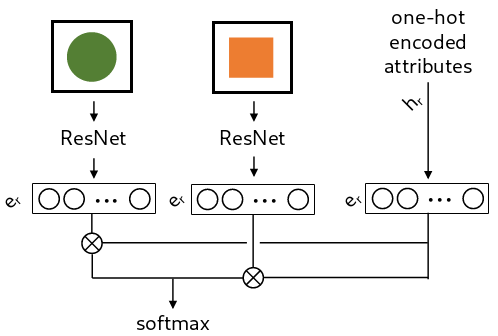
\includegraphics[width=.5\linewidth]{figures/arch_bounding_box_classifier.png}
    \caption{Simplified architecture of the object identification task}
    \label{fig:bounding_box_classifier_architecture}
    % SD: I haven't commented on this before, but let us be very careful in naming all meta-paramaters of the models in the text or in caption: how many layers, how many dimensions, etc. The reader should be able to replicate the code and the experiment from this. You can do this in the caption which is a longer explanation or in the text itself.
    % DK: TODO
\end{figure}

The model, the \textbf{object identifier} is split into three submodules, the \emph{bounding box encoder}, the \emph{attribute encoder} and the \emph{identifier}.
Each normalized bounding box of the sample is encoded with the \emph{bounding box encoder}.
Hereby, they are passed through \emph{ResNet-avg}.
The preceding layers \emph{ResNet-1} to \emph{ResNet-4} couldn't be compared due to memory restrictions on the GPU.
The resulting vector is flattened and projected to the embedding dimension $e$ via a linear layer.
% SD: This is quite low? Why only 10?
% DK: different embedding sizes are tested (done)
Correspondingly, the one-hot vector of the attributes is projected to the same embedding dimension with another linear layer, using the \emph{attribute encoder}.
In the \emph{identifier} submodule, each bounding box is combined with the representation of the attributes.
By bringing both vectors to the same embedding size, the dot product between each embedded bounding box and the embedded attributes can be calculated.
A high correlation between the attributes and the object should result in a high dot product, while a low correlation results in a lower dot product.
The model can so learn to connect the object representation with the attributes.
The dot products are concatenated and form a vector with as many dimensions as objects present.
The $softmax$ function is applied over the resulting vector, which returns a probability distribution over all objects; the model points to the object with the highest probability.
% The model then points to an object, using the \emph{softmax} function over this resulting vector.

The experiments are conducted with the following hyperparameters: a learning rate of $2\times10^{-4}$ and 30 epochs.
The number of epochs was chosen manually after identifying when the loss as well as the test accuracies didn't improve significantly.
The loss is calculated using cross entropy.
The following embedding dimension $e$ are compared: 2, 10, 50, 100, 500, 1000.
% SD: So, the output of this model is a vector of 0 and 1s, with the 1 identifying the corrct object (or the other way around?).
% DK: the output is a probability distriution over all objects (inserted above; done)

The object identification task is trained on all datasets that include more than one object in each sample, namely the 'CLEVR color', 'Dale-2' and 'Dale-5' dataset.
Random baselines for each dataset would yield accuracies of 10\%, 50\% and 20\% respectively.
% excluding the 'CLEVR single'.
% SD: Why not?
% DK: because there is only one object in the input, and therefore only one possible guess. The model can't point to a distractor (adressed; done)
The 'Dale' datasets are directly comparable to each other for the similar setup of their creation.
Especially interesting is the effect of the increasing the number of distractors and the growing number of attributes that are needed to discriminate the objects.

\subsubsection*{Results}
Table \ref{tab:results:bounding_box_classifier} lists the accuracies of the models' predictions after 30 epochs for all three different datasets and different embedding sizes $e$.

\begin{table}[ht]
    \centering
    \begin{tabular}{c|c|c|c}
        \toprule
               & \textbf{Dale-2}   & \textbf{Dale-5}   & \textbf{CLEVR Color} \\\cmidrule(lr){2-2}\cmidrule(lr){3-3}\cmidrule(lr){4-4}
        $e$    & \textbf{Accuracy} & \textbf{Accuracy} & \textbf{Accuracy}    \\\midrule
        {2}    & {92\%}            & {72\%}            & {40\%}               \\
        {10}   & \textbf{100\%}    & {94\%}            & {92\%}               \\
        {50}   & {99\%}            & \textbf{95\%}     & \textbf{94\%}        \\
        {100}  & \textbf{100\%}    & \textbf{95\%}     & {93\%}               \\
        {500}  & \textbf{100\%}    & \textbf{95\%}     & {93\%}               \\
        {1000} & \textbf{100\%}    & {94\%}            & \textbf{94\%}        \\
        \bottomrule
    \end{tabular}
    \caption{Accuracy scores of the object identifier after 30 epochs: $e$ are different embedding sizes}
    \label{tab:results:bounding_box_classifier}
\end{table}

The first trend that is visible is that fewer distractor increase the accuracy of the model.
The model achieves almost perfect accuracy in all configurations for the 'Dale 2' dataset with only two objects.
With five objects in the 'Dale-5' dataset, the accuracy drops to 95\% and with a maximum possible number of 10 objects in the 'CLEVR color' dataset the model only achieves 94\% in the best configuration.
This is not very surprising, since the model has a higher chance of predicting a wrong object, given the random baselines of 50\%, 20\% and 10\%.
Furthermore, when more objects are shown to the model, more attributes are needed to discriminate the target object from the distractor, since it is more likely that the distractors share attributes with the target object.
The task is getting therefore more challenging.

A second conclusion is that the model needs a certain embedding space, to represent the features of each image.
Across all dataset, an embedding space of only 2 dimensions result in a much lower performance compared to the best configuration.
Even though the model is still able to achieve an accuracy of 30\% to 50\% points over the random baseline, this shows that a bigger embedding size is beneficial to extract and represent the features of the objects.
Between 50 and 1000 dimensions, the model performs the best and varies only by 1\% point, which may be due to different random initialization of the weights in the model.

In conclusion, the model is able to learn to discriminate the objects based on the visual appearance.
The model can generate these high results, even with its relatively simple architecture.
In this architecture, the model doesn't compare the objects directly to each other, but each object is only associated with the attribute encodings.
A more complex architecture, in which the model is additionally tasked to discriminate the objects directly from each other might even improve the results.
% SD: The model is able to leatn to discriminate objects based on visual appearance.
% DK: (done)